\section{Results}
\label{sec:results}
% =============================================================

\textbf{A note on El~Paso.} A satellite-timestamp alignment bug --- a false
UTC offset on the raw ground-truth file, causing every satellite patch to
be paired with the wrong GHI label --- was found after the El~Paso figures
below were first computed. The ground-truth file has been corrected and
El~Paso retraining on it is in progress. Rather than omit El~Paso, every
value in this section derived from the pre-fix data is marked \dag\ and
reported as originally obtained; it should be read as pending
re-confirmation rather than as a final result, and will be updated as
corrected retraining completes (Section~\ref{sec:discussion}, Limitations).
Uniandes, SARIMA, and every ground-truth-only descriptive statistic in this
paper (Figures~\ref{fig:diurnal}--\ref{fig:delta-hist}, the example
satellite patch in Section~\ref{sssec:satellite}) are unaffected and
unmarked.

\subsection{Persistence reference}

Table~\ref{tab:persistence} reports the persistence $\rmseday$ at each site and
horizon, which defines the denominator of $\skillday$ for all models.

\begin{table}[t]
  \centering
  \caption{Persistence test-set $\rmseday$ (W/m²). All deep-learning models
           are compared against these values. El~Paso values (\dag) are
           pending re-confirmation (note above).}
  \label{tab:persistence}
  \begin{tabular}{lccc}
    \toprule
    \textbf{Site} & \textbf{1h} & \textbf{3h} & \textbf{6h} \\
    \midrule
    El Paso$^\dagger$   & 204.4 & 411.0 & 565.3 \\
    Uniandes  & 293.9 & 405.0 & 470.9 \\
    \bottomrule
  \end{tabular}
\end{table}

The 1-hour persistence error at El~Paso (204.4~W/m²$^\dagger$) is notably lower than at
Uniandes (293.9~W/m²), reflecting El~Paso's more stable clear-sky regime where
short-horizon irradiance changes are small --- a characterisation confirmed
independently from the corrected ground-truth record
(Figure~\ref{fig:delta-hist}). At 6~hours, both sites have comparable
absolute difficulty (565.3$^\dagger$ vs.\ 470.9~W/m²).

\FloatBarrier
\subsection{Main results}

Table~\ref{tab:main} reports $\rmseday$ and $\skillday$ for all models on the
test set. Deep-learning results are mean~$\pm$~std over four seeds.

\begin{table*}[t]
  \centering
  \caption{Test-set results. $\rmseday$ in W/m². $\skillday$ relative to persistence
           (higher is better). DL models: mean~$\pm$~std over 4 seeds.
           Best $\skillday$ per site-horizon highlighted in \textbf{bold}.
           El~Paso columns (\dag) were computed before a satellite-timestamp
           alignment bug was found and fixed and are pending re-confirmation
           on corrected data (note at the start of this section).}
  \label{tab:main}
  \setlength{\tabcolsep}{5pt}
  \resizebox{\textwidth}{!}{%
  \begin{tabular}{llcccccc}
    \toprule
    & & \multicolumn{3}{c}{\textbf{El Paso (César)$^\dagger$}} &
         \multicolumn{3}{c}{\textbf{Uniandes (Bogotá)}} \\
    \cmidrule(lr){3-5}\cmidrule(lr){6-8}
    \textbf{Model} & \textbf{Metric} & \textbf{1h} & \textbf{3h} & \textbf{6h}
                                     & \textbf{1h} & \textbf{3h} & \textbf{6h} \\
    \midrule
    \multirow{2}{*}{Persistence}
      & $\rmseday$ & 204.4 & 411.0 & 565.3  & 293.9 & 405.0 & 470.9 \\
      & $\skillday$ & 0.000 & 0.000 & 0.000 & 0.000 & 0.000 & 0.000 \\
    \midrule
    \multirow{2}{*}{ResNet-LSTM}
      & $\rmseday$ & $238.6 \pm 22.4$ & $238.5 \pm 42.7$ & $218.4 \pm 13.2$
                   & $246.7 \pm 4.1$ & $255.7 \pm 4.8$ & $297.9 \pm 8.8$ \\
      & $\skillday$ & $\mathbf{-0.167} \pm 0.110$ & $\mathbf{+0.420} \pm 0.104$ & $+0.614 \pm 0.023$
                    & $\mathbf{+0.161} \pm 0.014$ & $+0.369 \pm 0.012$ & $+0.368 \pm 0.019$ \\
    \midrule
    \multirow{2}{*}{GraphSAGE-LSTM}
      & $\rmseday$ & $244.7 \pm 8.1$ & $238.9 \pm 15.9$ & $\mathbf{206.1} \pm 7.4$
                   & $250.8 \pm 5.1$ & $252.5 \pm 1.5$ & $274.4 \pm 3.9$ \\
      & $\skillday$ & $-0.197 \pm 0.040$ & $+0.419 \pm 0.039$ & $\mathbf{+0.636} \pm 0.013$
                    & $+0.147 \pm 0.017$ & $\mathbf{+0.376} \pm 0.004$ & $\mathbf{+0.417} \pm 0.008$ \\
    \midrule
    \multirow{2}{*}{FlatMLP}
      & $\rmseday$ & --- & --- & --- & --- & --- & --- \\
      & $\skillday$ & --- & --- & --- & --- & --- & --- \\
    \bottomrule
  \end{tabular}}
  \par\smallskip
  \textit{\footnotesize GraphSAGE-LSTM rows use the \textbf{fixed unweighted
  graph} variant (Section~\ref{ssec:gsage}); results for the tuned weighted
  $k$-NN variant are in progress and reported separately in
  Table~\ref{tab:ablation}. FlatMLP results are pending completion of
  the four-seed sweep (Section~\ref{sec:discussion}, Limitations) and will be
  populated prior to submission; this row quantifies what fraction of
  deep-learning skill arises from spatial encoding versus temporal dynamics
  alone.}
\end{table*}

\begin{figure*}[t]
  \centering
  
\includegraphics[width=\textwidth]{figures/fig1_skill_day}
  \caption{Daytime skill score ($\skillday$) for ResNet-LSTM, GraphSAGE-LSTM
           (both Optuna-tuned, fixed-graph variant, four seeds), persistence,
           and SARIMA, at both sites across three forecast horizons. Bars show
           mean over four seeds; error bars indicate $\pm 1$ standard
           deviation. Persistence has no seed variability. The hatched SARIMA
           bars use the rolling-origin protocol of Section~\ref{ssec:sarima},
           are evaluated on a coarser, on-the-hour subset of the test set
           against a smoother hourly-mean target, with their own recomputed
           persistence reference, and are \textbf{not directly comparable}
           to the other bars; FlatMLP is omitted pending completion of its
           Optuna sweep (Section~\ref{sec:discussion}, Limitations). El~Paso's
           ResNet-LSTM/GraphSAGE-LSTM bars are not shown here: their pre-fix
           values were invalidated by the satellite-timestamp bug (note at
           the start of this section) and are not reproduced in this figure,
           pending corrected retraining; the corresponding pre-fix number
           ($0.636^\dagger$, Table~\ref{tab:main}) is reported in text only.
           GraphSAGE-LSTM achieves the highest skill among the deep-learning
           models at the 6-hour horizon at Uniandes ($0.417$), the only site
           shown here with currently-valid deep-learning results.}
  \label{fig:skill}
\end{figure*}

\begin{figure*}[t]
  \centering
  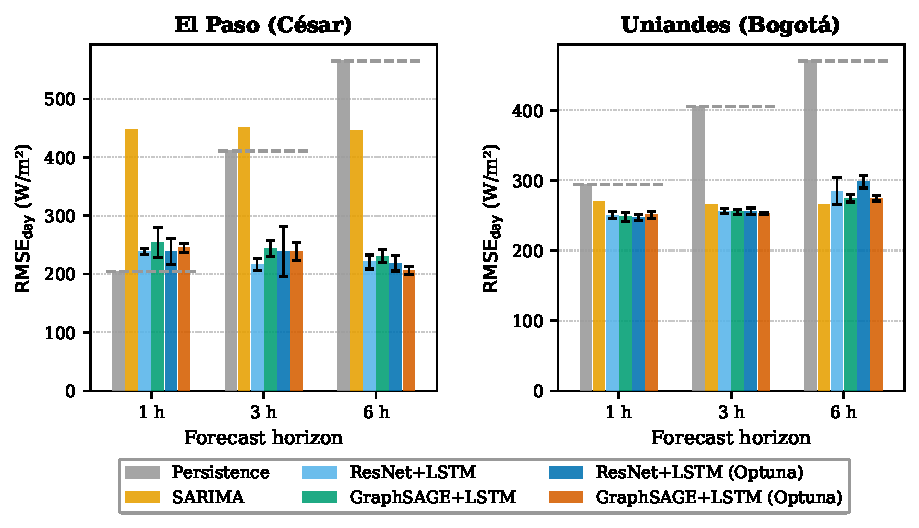
\includegraphics[width=\textwidth]{figures/fig2_rmse_day}
  \caption{Daytime RMSE ($\rmseday$, W/m²) for ResNet-LSTM, GraphSAGE-LSTM,
           persistence, and SARIMA. Dashed horizontal lines show the
           persistence reference for each horizon group. The hatched SARIMA
           bars use a coarser on-the-hour test subset and are
           \textbf{not directly comparable} to the other bars
           (Section~\ref{ssec:sarima}); FlatMLP is omitted pending completion
           of its Optuna sweep. As in Figure~\ref{fig:skill}, El~Paso's
           ResNet-LSTM/GraphSAGE-LSTM bars are withheld pending corrected
           retraining (note at the start of this section); only Persistence
           and SARIMA are currently valid for that site. At Uniandes, both
           Optuna-tuned deep-learning models substantially reduce RMSE
           relative to persistence at 3h and 6h, with GraphSAGE-LSTM
           achieving the lowest RMSE at the 6-hour horizon.}
  \label{fig:rmse}
\end{figure*}

\paragraph{SARIMA reference.}
Under the rolling-origin protocol of Section~\ref{ssec:sarima}, SARIMA
attains substantial positive skill against its own on-the-hour persistence
reference at every horizon at both sites (El~Paso: $0.42$/$0.65$/$0.74$ at
1h/3h/6h; Uniandes: $0.33$/$0.41$/$0.48$), growing with horizon: with daily
seasonal differencing, the model anticipates the diurnal ramp that
persistence, by construction, cannot, and this advantage is largest exactly
where persistence degrades most. These skill values are \emph{not}
directly comparable to Table~\ref{tab:main}: SARIMA is evaluated on the
on-the-hour subset only and, more importantly, forecasts hourly-\emph{mean}
GHI --- a target from which the within-hour 10-minute variability the
deep-learning models must resolve has been averaged out --- so its lower
$\rmseday$ partly reflects a smoother target rather than superior
short-timescale forecasting. A like-for-like comparison (deep-learning
models re-evaluated on the same hourly-mean, on-the-hour basis) is left for
future work; within this paper SARIMA serves as a classical reference
demonstrating how much of the horizon-dependent skill is attributable to
diurnal-cycle structure alone, without any satellite information.

\FloatBarrier
\subsection{Graph-construction ablation: fixed vs.\ tuned spatial connectivity}
\label{ssec:ablation}

Table~\ref{tab:ablation} isolates the contribution of \emph{tuned spatial
connectivity} by comparing the fixed unweighted 8-neighbour graph (used for
the GraphSAGE-LSTM rows of Table~\ref{tab:main}) against the tuned,
distance-weighted $k$-nearest-neighbour graph with Optuna-tuned neighbourhood
size $k$ (Section~\ref{ssec:gsage}), holding the rest of the architecture,
training protocol, and data pipeline fixed. The weighted-graph variant uses a
reduced two-seed protocol (Section~\ref{ssec:optuna}); we report it alongside
the four-seed fixed-graph baseline with this caveat rather than withholding
it pending a full four-seed re-run.

\begin{table*}[t]
  \centering
  \caption{Graph-construction ablation for GraphSAGE-LSTM. $\skillday$ relative
           to persistence (higher is better). Fixed graph: mean~$\pm$~std over
           4 seeds. Weighted $k$-NN graph: mean~$\pm$~std over 2 seeds
           $\{42,1\}$ (Section~\ref{ssec:optuna}). El~Paso column (\dag) is the
           pre-fix fixed-graph result (note at the start of Section~\ref{sec:results});
           its weighted $k$-NN counterpart will be reported once corrected
           retraining completes, with no fixed-vs-tuned ablation at that site
           until then (Section~\ref{sec:discussion}, Limitations).
           \textit{[Weighted $k$-NN ablation in progress; values to be
           populated as runs complete.]}}
  \label{tab:ablation}
  \setlength{\tabcolsep}{5pt}
  \resizebox{\textwidth}{!}{%
  \begin{tabular}{llcccccc}
    \toprule
    & & \multicolumn{3}{c}{\textbf{El Paso (César)$^\dagger$}} &
         \multicolumn{3}{c}{\textbf{Uniandes (Bogotá)}} \\
    \cmidrule(lr){3-5}\cmidrule(lr){6-8}
    \textbf{Graph variant} & \textbf{Metric} & \textbf{1h} & \textbf{3h} & \textbf{6h}
                                              & \textbf{1h} & \textbf{3h} & \textbf{6h} \\
    \midrule
    Fixed unweighted, $k=8$ (4 seeds)
      & $\skillday$ & $-0.197 \pm 0.040$ & $+0.419 \pm 0.039$ & $+0.636 \pm 0.013$
                    & $+0.147 \pm 0.017$ & $+0.376 \pm 0.004$ & $+0.417 \pm 0.008$ \\
    \midrule
    \multirow{2}{*}{Weighted $k$-NN, tuned (2 seeds)}
      & $\skillday$ & --- & --- & --- & --- & --- & --- \\
      & best $k$ & --- & --- & --- & --- & --- & --- \\
    \bottomrule
  \end{tabular}}
\end{table*}

\subsection{Horizon-by-horizon analysis}

\paragraph{1-hour horizon.}
Both deep-learning models fail to beat persistence at El~Paso (Figure~\ref{fig:skill}): ResNet-LSTM
($\skillday = -0.167^\dagger \pm 0.110$) and GraphSAGE-LSTM ($-0.197^\dagger \pm 0.040$) show
negative skill, meaning they produce higher RMSE than simply repeating the last
observation. At Uniandes the picture is more favourable: ResNet-LSTM achieves
modest positive skill ($+0.161 \pm 0.014$), narrowly ahead of GraphSAGE-LSTM
($+0.147 \pm 0.017$). The key difference between sites is the persistence
reference: El~Paso's 1-hour persistence RMSE (204.4~W/m²$^\dagger$) is comparatively low
because irradiance changes slowly under predominantly clear-sky conditions,
leaving little room for improvement from data-driven methods. Uniandes' 1-hour
persistence RMSE (293.9~W/m²) is higher due to the frequent cloud passages,
which create more structure for the models to exploit. This is consistent
with the raw GHI series itself: its autocorrelation decays faster at
Uniandes than at El~Paso at every lag up to 6~hours (Figure~\ref{fig:acf}),
so the most recent observation --- what persistence relies on --- is a
comparatively weaker predictor there.

\begin{figure}[t]
  \centering
  \includegraphics[width=\columnwidth]{fig5_acf_ghi}
  \caption{Autocorrelation of the raw 10-minute GHI series up to a 6-hour
           lag, both sites. Faster decay at Uniandes reflects its more
           variable cloud cover and explains its higher persistence RMSE
           at every horizon (Table~\ref{tab:persistence}).}
  \label{fig:acf}
\end{figure}

\paragraph{3-hour horizon.}
Both deep-learning models outperform persistence at El~Paso by approximately
42\%$^\dagger$ ($\skillday \approx 0.42^\dagger$ for both architectures: $+0.420^\dagger \pm 0.104$ for
ResNet-LSTM versus $+0.419^\dagger \pm 0.039$ for GraphSAGE-LSTM, a difference well
within one standard deviation and therefore not distinguishable at this
horizon). The large standard deviation for ResNet-LSTM ($\pm 0.104$) reflects
seed-to-seed variability, with some seeds achieving near-GraphSAGE performance
and others considerably below.

At Uniandes, GraphSAGE-LSTM attains the best skill at this horizon
($+0.376 \pm 0.004$), narrowly ahead of ResNet-LSTM ($+0.369 \pm 0.012$); both
are similar to each other and slightly below their El~Paso counterparts despite
the higher absolute persistence error at this site.

\paragraph{6-hour horizon.}
This is the most favourable horizon for the deep-learning models
(Figures~\ref{fig:skill}--\ref{fig:rmse}).
\textbf{GraphSAGE-LSTM achieves the best overall result}: $\rmseday = 206.1^\dagger \pm 7.4$~W/m²
and $\skillday = 0.636^\dagger \pm 0.013$ at El~Paso, reducing the persistence RMSE by
63.6\%$^\dagger$. ResNet-LSTM is close ($0.614^\dagger \pm 0.023$) but consistently below GraphSAGE
across all seeds.

At Uniandes, GraphSAGE-LSTM again leads ($0.417 \pm 0.008$ vs.\ $0.368 \pm
0.019$ for ResNet-LSTM), with a wider margin than at El~Paso (+0.049 vs.\
+0.022$^\dagger$ percentage points of skill). However, the \emph{absolute} skill at
Uniandes remains markedly lower than at El~Paso for both architectures ---
the gap we analyse in Section~\ref{sec:discussion}.

\begin{figure}[t]
  \centering
  \fbox{\begin{minipage}[c][0.28\textheight][c]{0.9\columnwidth}
    \centering\small
    \textit{Figure pending regeneration.}\\[4pt]
    This panel showed a five-day excerpt of the 6-hour GHI forecast from
    GraphSAGE-LSTM (fixed-graph, seed~42) at El~Paso in January 2024, computed
    before the satellite-timestamp alignment bug (Section~\ref{sec:results}
    note; Section~\ref{sec:discussion}, Limitations) was found. Because every
    point in that timeseries is a specific (satellite, GHI) pairing rather
    than an aggregate statistic, the pre-fix version is not reproduced here;
    it will be regenerated once El~Paso retraining on the corrected
    ground-truth completes.
  \end{minipage}}
  \caption{[Placeholder] Five-day excerpt of the 6-hour GHI forecast from the
           best model (GraphSAGE-LSTM, fixed-graph, seed~42) at El~Paso,
           pending regeneration on corrected data --- see note above.}
  \label{fig:ts}
\end{figure}

\subsection{Statistical robustness}

The standard deviation across seeds provides a measure of training stability.
GraphSAGE-LSTM consistently shows lower seed-to-seed variability than ResNet-LSTM
(e.g., El~Paso 6h$^\dagger$: $\pm 0.013$ vs.\ $\pm 0.023$), suggesting that the graph
structure regularises training and reduces sensitivity to weight initialisation.
The most unstable model is ResNet-LSTM at El~Paso 3h$^\dagger$ ($\pm 0.104$), which may
reflect the interaction between the high-irradiance regime and the CNN's sensitivity
to specific initialisation-driven features.

\subsection{Epistemic uncertainty quantification}
\label{ssec:uq_results}

Table~\ref{tab:decomposition} will report the SGLD-based epistemic
uncertainty (Eq.~\ref{eq:epistemic}) for the best-performing backbone at
each site-horizon combination, together with the predictive interval's
empirical coverage at nominal levels 80\%, 90\%, and 95\%. $\sigma_\text{epi}$
(W/m²) is the spread of the $T$ posterior point predictions and shrinks as
more representative training data is available; it does not capture the
irreducible aleatoric noise of cloud stochasticity, so the resulting
interval should be read as a lower bound on total predictive uncertainty
(Section~\ref{sec:discussion}, Limitations).

The backbone for El~Paso is GraphSAGE-LSTM (best overall model at 3h and 6h
in the fixed-graph baseline, Table~\ref{tab:main}); for Uniandes the best
deep-learning backbone per horizon is used (ResNet-LSTM at 1h, GraphSAGE-LSTM
at 3h and 6h). The backbone selection will be revisited once the
graph-construction ablation (Table~\ref{tab:ablation}) completes, in case the
weighted $k$-NN variant supersedes the fixed-graph baseline used here.

\begin{table*}[t]
  \centering
  \caption{SGLD-based epistemic uncertainty. $\sigma_\text{epi}$ in W/m²
           (Eq.~\ref{eq:epistemic}); $\hat{\text{cov}}_\text{day}$: empirical
           daytime coverage of the interval $\bar\mu \pm z_{1-\alpha/2}\sigma_\text{epi}$
           on the test set. Backbone: GraphSAGE-LSTM for El~Paso; best-per-horizon
           deep-learning backbone for Uniandes (ResNet-LSTM at 1h, GraphSAGE-LSTM
           at 3h and 6h). \textit{[SGLD sampling in progress; values to be
           populated as runs complete.]}}
  \label{tab:decomposition}
  \setlength{\tabcolsep}{4pt}
  \resizebox{0.6\textwidth}{!}{%
  \begin{tabular}{llcc}
    \toprule
    \textbf{Site} & \textbf{H} &
    $\sigma_\text{epi}$ & $\hat{\text{cov}}_\text{day}$ (90\%) \\
    \midrule
    El Paso  & 3h & --- & --- \\
    El Paso  & 6h & --- & --- \\
    \midrule
    Uniandes & 1h & --- & --- \\
    Uniandes & 3h & --- & --- \\
    Uniandes & 6h & --- & --- \\
    \bottomrule
  \end{tabular}}
\end{table*}
